
\chapter{Introduction}
\label{chapter:intro}
\minitoc
\bigskip


% I like the introduction of the thesis of ZUCKER (but very short) : http://www.cs.cmu.edu/~mzucker/mz-thesis.pdf
\begin{figure}[h]
    \centering
    \captionsetup[subfigure]{justification=centering}
    \begin{subfigure}[t]{0.48\linewidth}
        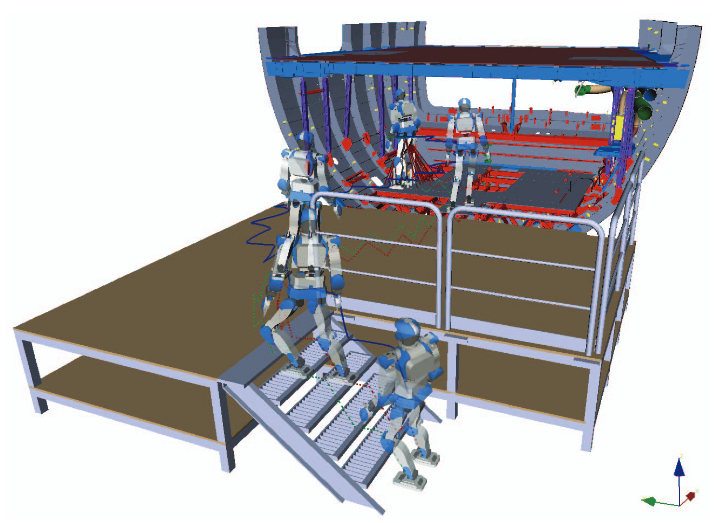
\includegraphics[width=\textwidth,height=5cm]{Figures/Chapter_INTRO/caron_image_plane.png}
        \caption{}
        \label{fig:intro_0}
    \end{subfigure}
    %\begin{subfigure}[t]{0.48\linewidth}
    %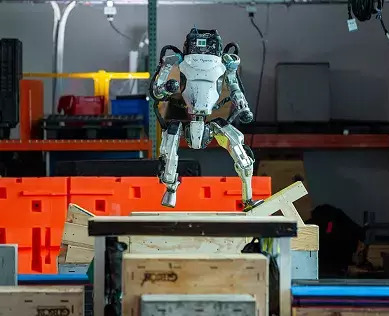
\includegraphics[width=\textwidth,height=5cm]{Figures/Chapter_INTRO/atlas_boston_dynamics.jpg}
    %\caption{\label{fig:intro_1}}
    %end{subfigure}
    \begin{subfigure}[t]{0.48\linewidth}
        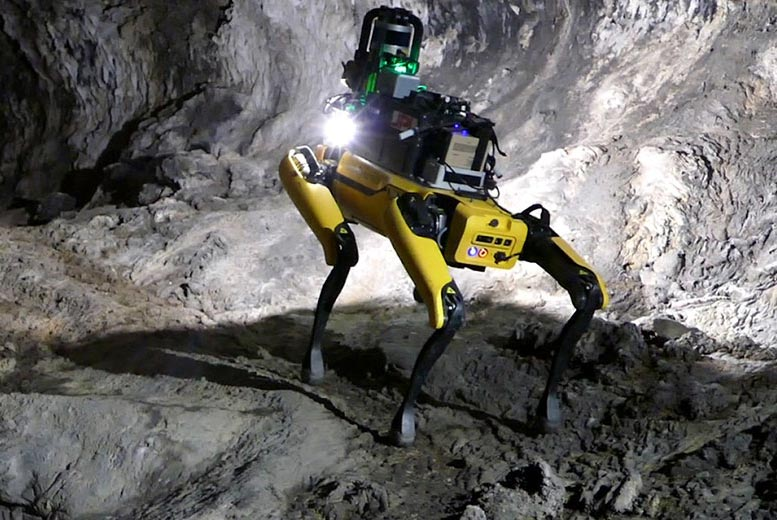
\includegraphics[width=\textwidth,height=4.5cm]{Figures/Chapter_INTRO/darpa_nasa.jpg}
        \caption{}
        \label{fig:intro_1}
    \end{subfigure}
    %\caption{Legged robots locomotion in complex environments. Sources: (a) \copyright Boston Dynamics and (b) \copyright NASA/JPL-Caltech.\label{fig:intro}}
    %\caption{Legged robots locomotion in complex environments. Sources: Caron et al. \cite{caron_plane_2016} and (b) ATLAS robot \copyright Boston Dynamics.\label{fig:intro}}
    \caption{Legged robots are currently opening a new area of robotics capabilities, beyond what wheeled manipulators are able to reach, in many domains such as aerospace manufacturing or underground exploration... and later in our homes? Sources: (a) Caron et al. \cite{caron_plane_2016} and (b) \copyright NASA/JPL-Caltech.}
    \label{fig:intro}
\end{figure}

% TITLE: Reinforcement Learning of a Navigation Method for Contact Planning on Humanoid Robots


%    What is the problem?
%    Why is it interesting and important?
%    Why is it hard? (E.g., why do naive approaches fail?)
%    Why hasn't it been solved before? (Or, what's wrong with previous proposed solutions? How does mine differ?)
%    What are the key components of my approach and results? Also include any specific limitations. 

% https://www.futura-sciences.com/tech/actualites/robotique-interview-construire-robots-humanoides-90953/ : 
% Un des principaux intérêts motivant la construction de robots humanoïdes est sans doute sa compatibilité avec le monde des humains. Sans adaptation de notre environnement, ils pourraient vivre en harmonie avec nous au quotidien pour nous aider et utiliser nos infrastructures.

Robots are already essential tools in the industry and will play a part in our daily life in the near future.
However, most of them still require specifically designed environments to perform their task.
In recent years, research on legged robots has opened a whole new range of possibilities. %in primarily human-made environments.
These robots could operate in less structured industrial areas to perform various tasks just like us (Figure \ref{fig:intro_0}). They could also explore in our stead risky environments as demonstrated during the DARPA subterranean challenge \cite{darpa_nasa_2021, darpa_hutter_2022}, where the robots have to map, navigate, and search for casualties in complex underground environments (Figure \ref{fig:intro_1}).

Nevertheless, to achieve these tasks, they have yet to perform the most basic but challenging skill that is to \textit{locomote through the environment}.

\section{Legged locomotion in complex environments}
% Je veux refaire le raisonnement de ce qu'un humain fait pour se mouvoir.
\begin{figure}[h]
    \centering
    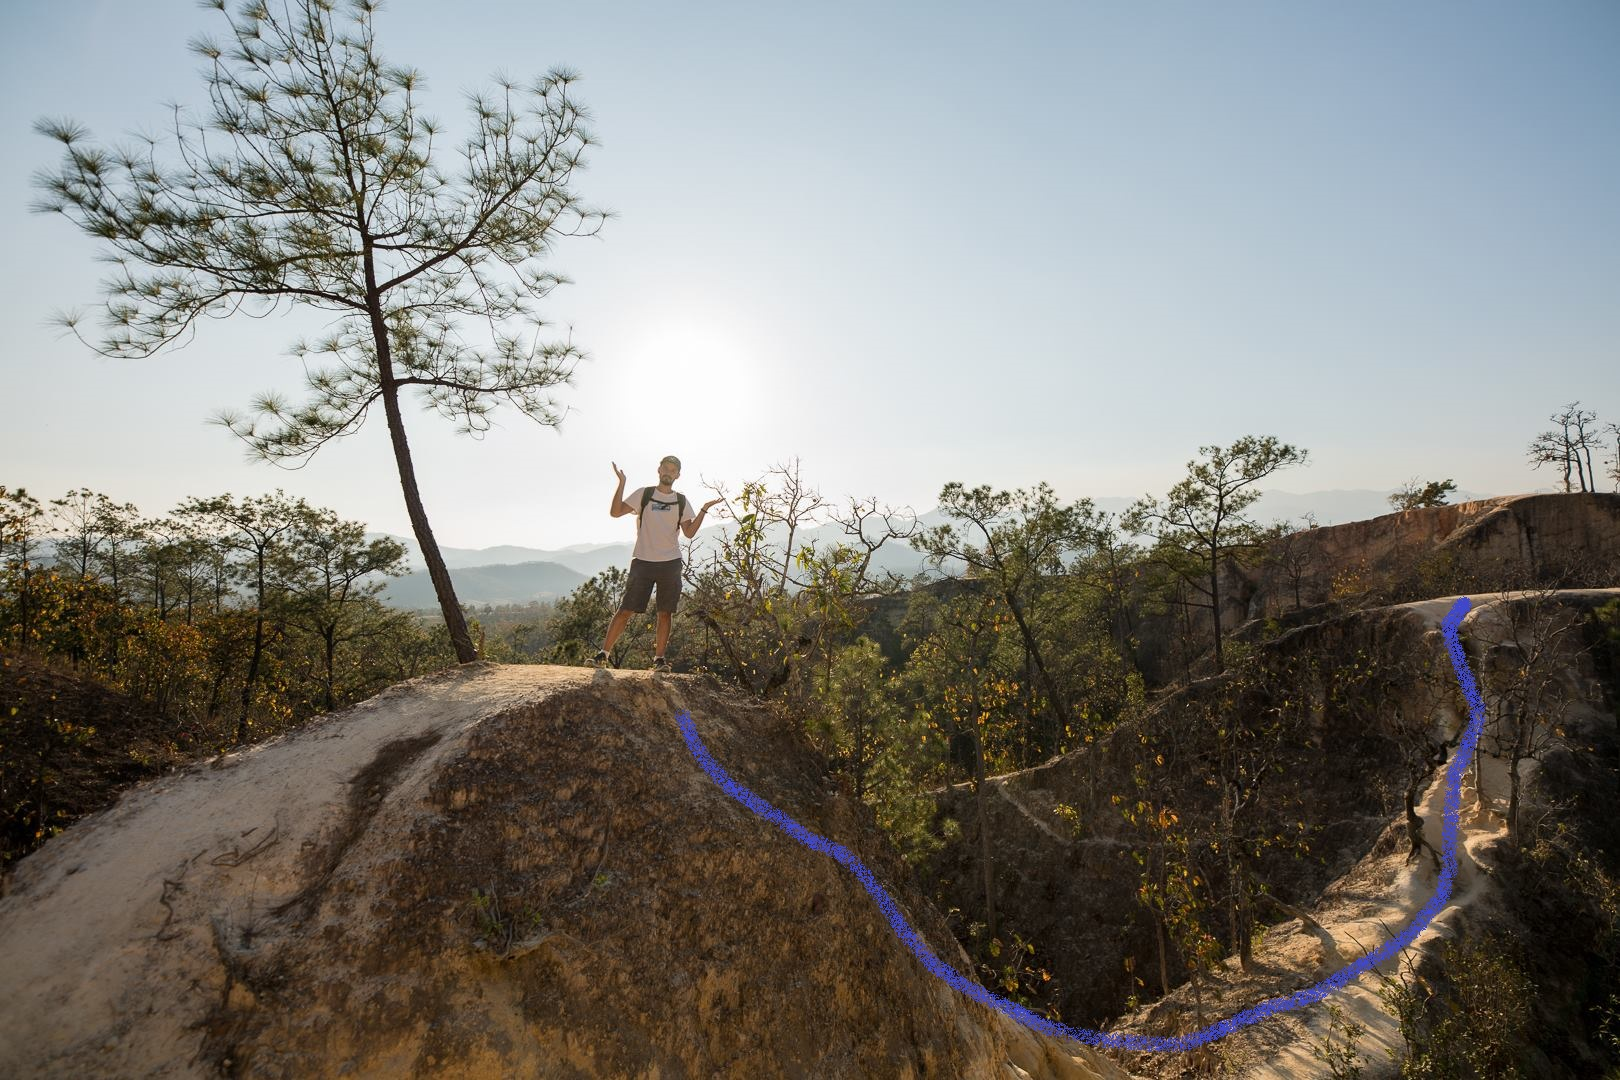
\includegraphics[width=\textwidth, height=8cm, trim={10cm 0 0 8cm}, clip]{Figures/Chapter_INTRO/moi_chemin.jpg}
    \caption{Planning the path is crucial for locomotion on complex terrains. While the blue trajectory is likely an easy output of our supercomputer human brain, asserting its feasibility can yet only be achieved by actually walking the path with our body.}
    \label{fig:intro:moi_chemin}
\end{figure}
In the large collection of works on legged robots, several strategies emerged to solve this problem.
In this thesis, we are interested in the robot locomotion problem in complex environments, that can be solved with a similar decision process to their creators.

We humans can achieve this task in real-time. 
As shown in Figure \ref{fig:intro:moi_chemin}, the objective is as follows: \qq{how to reach the other side of this terrain?}
Here, this task is particularly difficult, hence thorough planning is required.
We can typically decompose this task into two sub-problems:
\begin{enumerate}
    \item \textit{What path do we take?} 
    This decision is based on an estimation of our capabilities. 
    First, the path is subject to conditions of \textit{reachability}, as we need to be able to touch the ground, and obviously of \textit{collision avoidance} as we can not go through obstacles.
    Second, we need to evaluate the terrain \textit{traversability} to plan a feasible path. 
    Based on these criteria, we decide to plan the blue path in our example.
    \item \textit{How do we move our body to follow the path?} 
    Walking without thinking about where to place my foot could be sufficient for most scenarios. However, difficult terrains such as this one require a careful \textit{contact planning} to avoid taking a wrong step and falling.
\end{enumerate}
Following our human intuition, we approach these questions in two stages with (1) a navigation task to plan a feasible path, and (2) walking along this path while carefully planning our contact on the terrain.

% Added by nico
The key difficulty is that the two stages are intricate, as the only complete way to solve (1) is to also solve (2).
Again, we can have the intuition that our brain works with simplified models representing feasible solutions of (2) when exploring the candidate paths in (1).

%Legged robot locomotion in general can employ the same strategy as demonstrated during the DARPA subterranean challenge \cite{darpa_nasa_2021, darpa_hutter_2022}.In disaster scenarios, the robots have to map, navigate, and search for casualties in complex underground environments.

However, reproducing the masterful human reasoning for locomotion remains yet a difficult problem. How to program robots to achieve this decision process?
%Furthermore, this decision process changes from individual to individual who continuously learns to estimate and improve their capabilities.
Furthermore, can we automatically deduce navigation models handling the first stage (1), from the empirical capabilities of the contact planner (2), with the hope to extend them to other robot morphologies or capabilities?



\section{Thesis Statement and Summary}

%This thesis if part of the Loco3D project \cite{loco3d} which goal is to achieve a fast to compute and safe solution for legged robot locomotion in complex environments.
%In this context, we will further explored the use of a navigation task prior to contact planning on the terrain.
%Our research topic is the critical limitation of this approach, that is the path feasibility by a contact planner.

% By nico
This thesis builds upon the so-called Loco3D framework \cite{loco3d, thesis_steve} whose goal is to achieve a fast computing and safe solution for legged robot locomotion in complex environments.
At the core of the locomotion workflow is a clever model of the robot locomotion capabilities, the reachability model \cite{RB-PRM}, used to simplify the legged navigation planning. We will discuss the importance of this model in locomotion planning, but also its limitations in the next chapter.

Our research topic is to provide a better alternative to this model by replacing the human intuition used to design it with a systematic evaluation of the robot locomotion feasibility based on data generation and machine learning.

Our main contribution is a local navigation method learned by reinforcement. 
Our method, named LEAS, can locally navigate under reachability and collision-avoidance constraints using a local observation of its environment.
%During training time, LEAS can be plugged into a contact planner to learn how to generate more likely feasible paths for it, hence approximating its capabilities.
%Finally, we will connect our navigation method with 3 different contact planners from the Loco3D project.

%\hfill \break
\hfill \break

The organization of this thesis is as follows:

Chapter \ref{sec:sota} presents a review of the works on legged robot locomotion. 
We explore different solutions to obtain a safe and robust locomotion, leading us to our choice of a navigation method prior to contact planning (also known as the motion-before-contact approach), from which we formulate our main contribution.
%Finally, we present a general literature overview of the methods used in navigation that inspired our solution.


Chapter \ref{sec:LEAS} presents our steering method LEAS, that can locally navigate complex terrains.
We describe our method to learn by reinforcement how to generate paths under reachability and collision-avoidance constraints.
%This chapter presents LEAS without being plugged to a contact planner, which is a local navigation task in 3D.
The capabilities of LEAS are then empirically explored, exemplified, and characterized using a simple feasibility oracle.

Chapter \ref{sec:CP-SB} presents the results of LEAS using the acyclic sampling-based contact planner \cite{AcyclicCP} as a feasibility oracle.
Our steering method learns how to generate paths fitting this contact planner. 
%As a result, it solves the compatibility problem we had with our previous solutions between navigation and contact planning.
With this setting, LEAS can improve the performance of the planner using the reachability condition, without requiring the tuning of the intuition-based model.

Chapter \ref{sec:CP-SL1M} generalizes the training of LEAS with the more advanced contact planners, MIP and SL1M \cite{sl1m_v2}.
%investigates the use of LEAS plugged into the Mixed-Integer Programming contact planner and its relaxation \cite{sl1m_v2}. 
We explain their formulation and their limitations relative to the path. Finally, we present the current results as well as the different experiments we conducted.

Chapter \ref{sec:conclusion} discusses the advantages and limitations of our steering method, finally concluding with the perspective of our work.